\subsubsection{Moduł komunikacyjny}
Struktura:
\begin{itemize}
	\item storage/src/dist/storage\_dist\_srv.erl – gen\_server
\end{itemize}
Jest to moduł odpowiedzialny za komunikację między węzłami systemu. Zapytania generowane przez bibliotekę kliencką trafiają właśnie tutaj. Są autentykowane a następnie przesyłane dalej zgodnie z polityką obsługi danego typu zapytania.

gen\_server w swoim stanie przechowuje zbiór adresów wszystkich węzłów w systemie (rezultat wywołania node() na każdym węźle). Standardowy protokół tworzenia i aktualizacji tego zbioru opisuje rozdział Dołączanie węzłów (synchronizacja stanu).

\begin{figure}[!htbp]
	\centering
	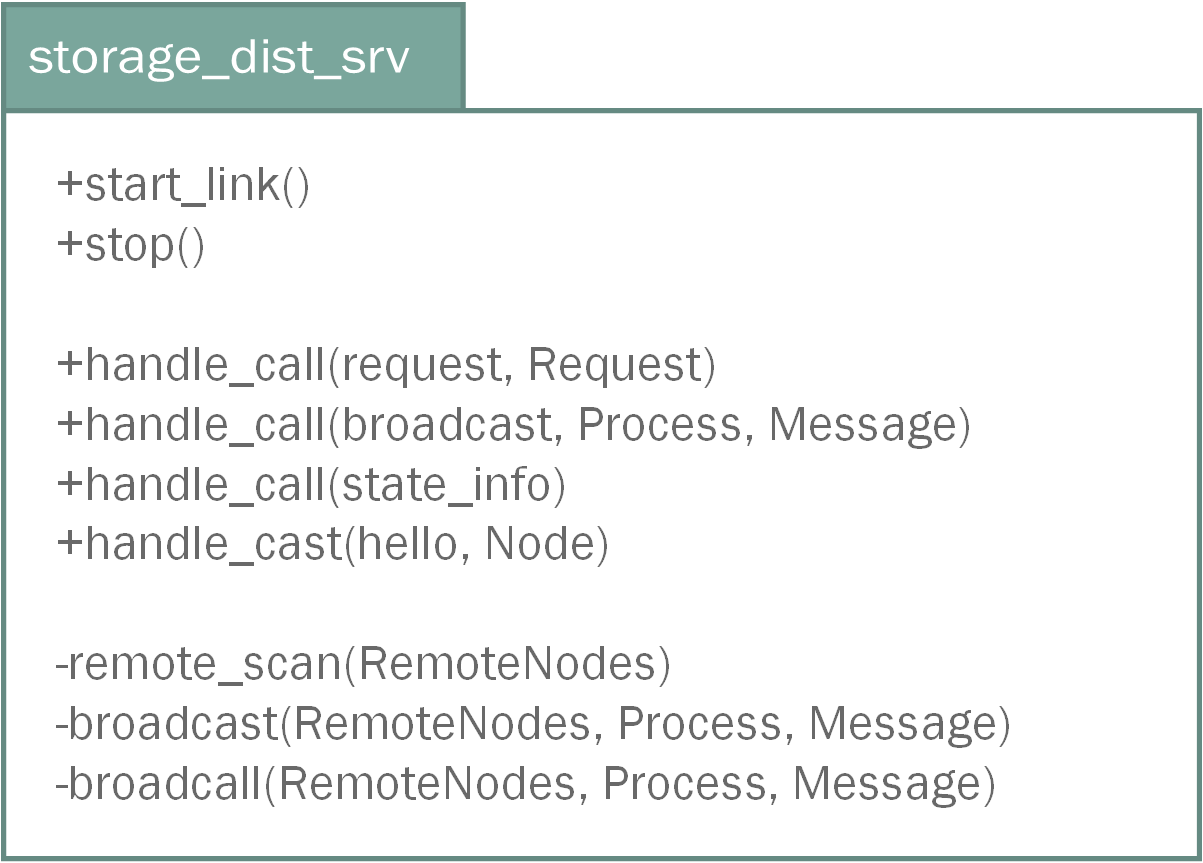
\includegraphics[width=0.7\textwidth]{dist-module}
	\caption[Struktura modułu komunikacyjnego.]{Publiczny interfejs modułu storage\_dist\_srv. Podstawowa metoda to handle\_call(request, Request), która jest zdalnie wywoływana przez API klienckie z odpowiednią strukturą zapytania jako argument.}
	\label{fig:dist-module}
\end{figure}

\paragraph{Obsługa zapytań read, delete, find} Wszystkie te zapytania obsługiwane są w identyczny sposób. Przykładowy ciąg sekwencji przy obsłudze zapytania typu read (rozsyłanego do wszystkich węzłów) przedstawia \autoref{fig:dist-seq}.

Źródłem zapytania jest proces używający biblioteki klienckiej (client), wywołujący synchroniczne zapytanie na module storage\_dist\_srv. Od razu tworzony jest nowy proces odpowiedzialny za obsługę tego żądania. Główny proces gen\_servera zwraca z handle\_call status noreply i kontynuuje działanie. Wygenerowanie odpowiedzi i przesłanie jej do użytkownika będzie należało do jednego z modułów storage\_core\_srv, gdzie przesłana jest odpowiednia struktura Request.

Proces obsługi zapytania autentykuje je przy użyciu modułu storage\_auth\_srv zaraz po jego otrzymaniu.

\begin{figure}[!htbp]
	\centering
	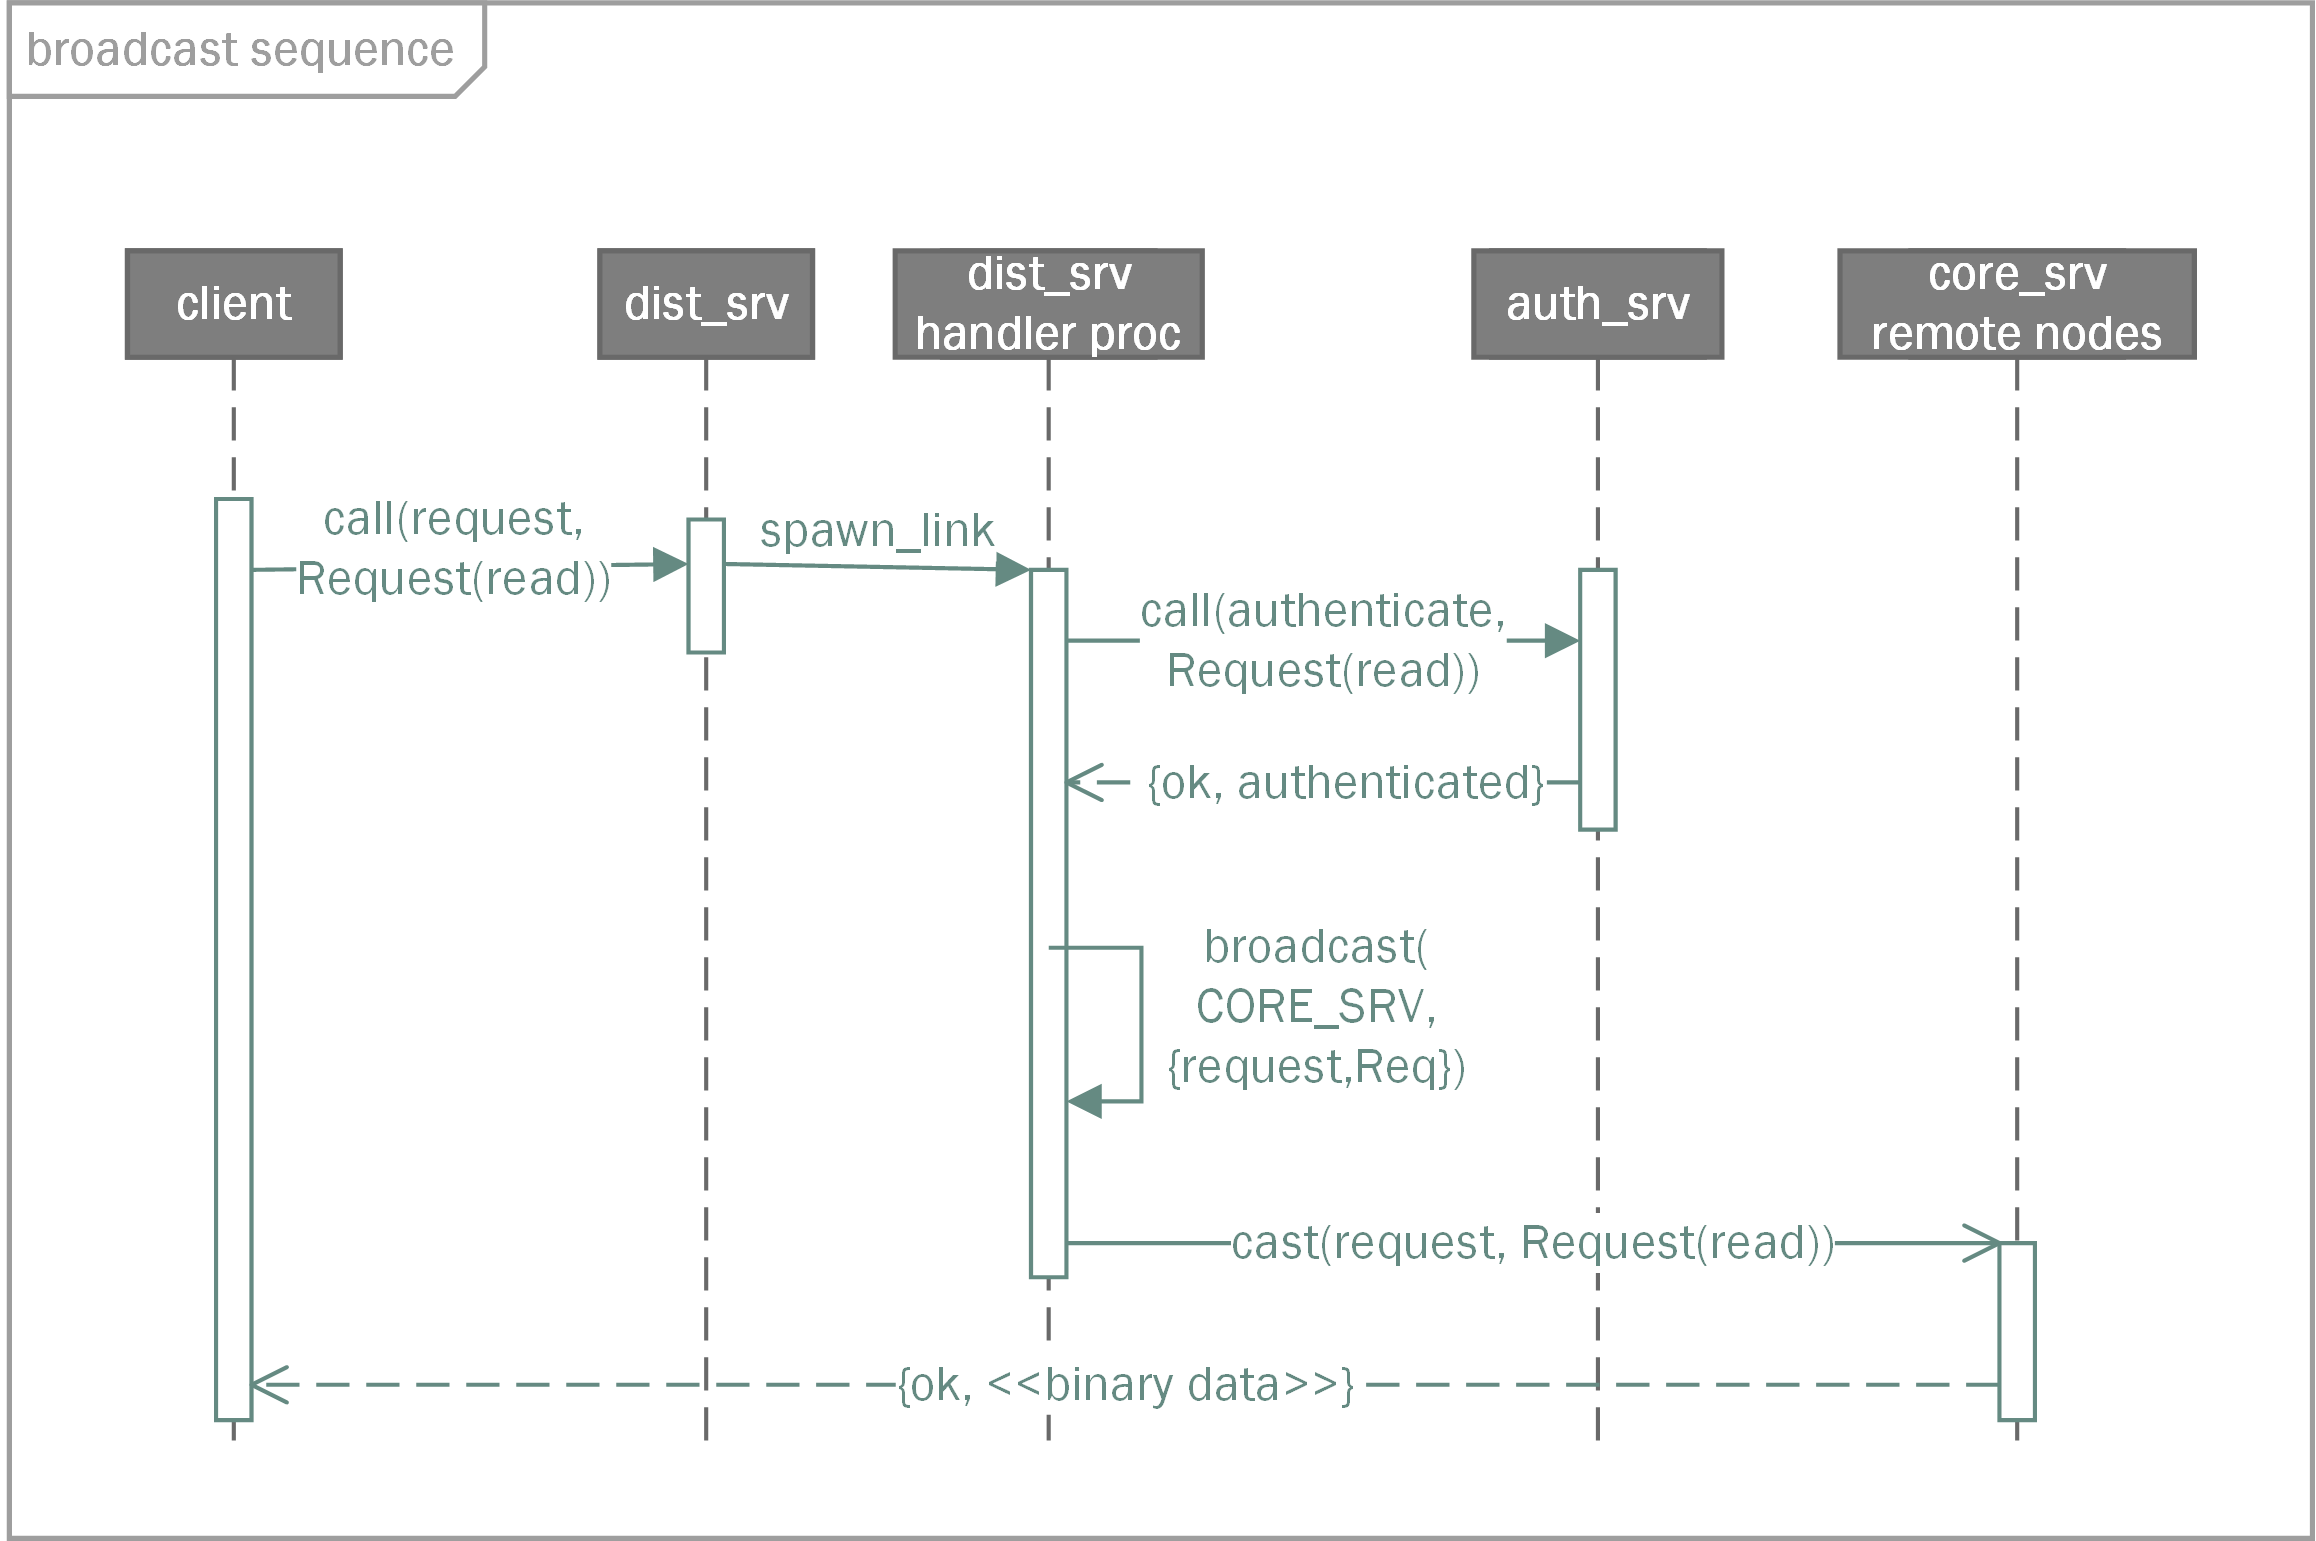
\includegraphics[width=0.9\textwidth]{dist-seq}
	\caption[Zapytanie \textit{read} w module komunikacyjnym.]{Sekwencja wywołań przy obsłudze zapytania read w module storage\_dist\_srv.}
	\label{fig:dist-seq}
\end{figure}

\paragraph{Obsługa zapytań create}
Zapytanie create różni się od obsługi zapytań read, delete czy find. Wymaga zlokalizowania węzła o najmniejszym zapełnieniu, który może pomieścić dany plik. Do modułów storage\_core\_srv na wszystkich węzłach w systemie wysyłana jest wiadomość {reserve, Size}, gdzie Size jest rozmiarem pliku. Jeżeli dany węzeł może przyjąć plik, odpowiada komunikatem {ok, Fill}, gdzie Fill jest jego procentowym zapełnieniem. Do niego następnie przesyłane jest właściwe żądanie użytkownika. Do pozostałych węzłów trafia komunikat {release, Size}, mówiący, że mogą zwolnić zarezerwowane zasoby dyskowe. Sekwencja wywołań przedstawiona jest na \autoref{fig:dist-create-seq}.

\begin{figure}[!htbp]
	\centering
	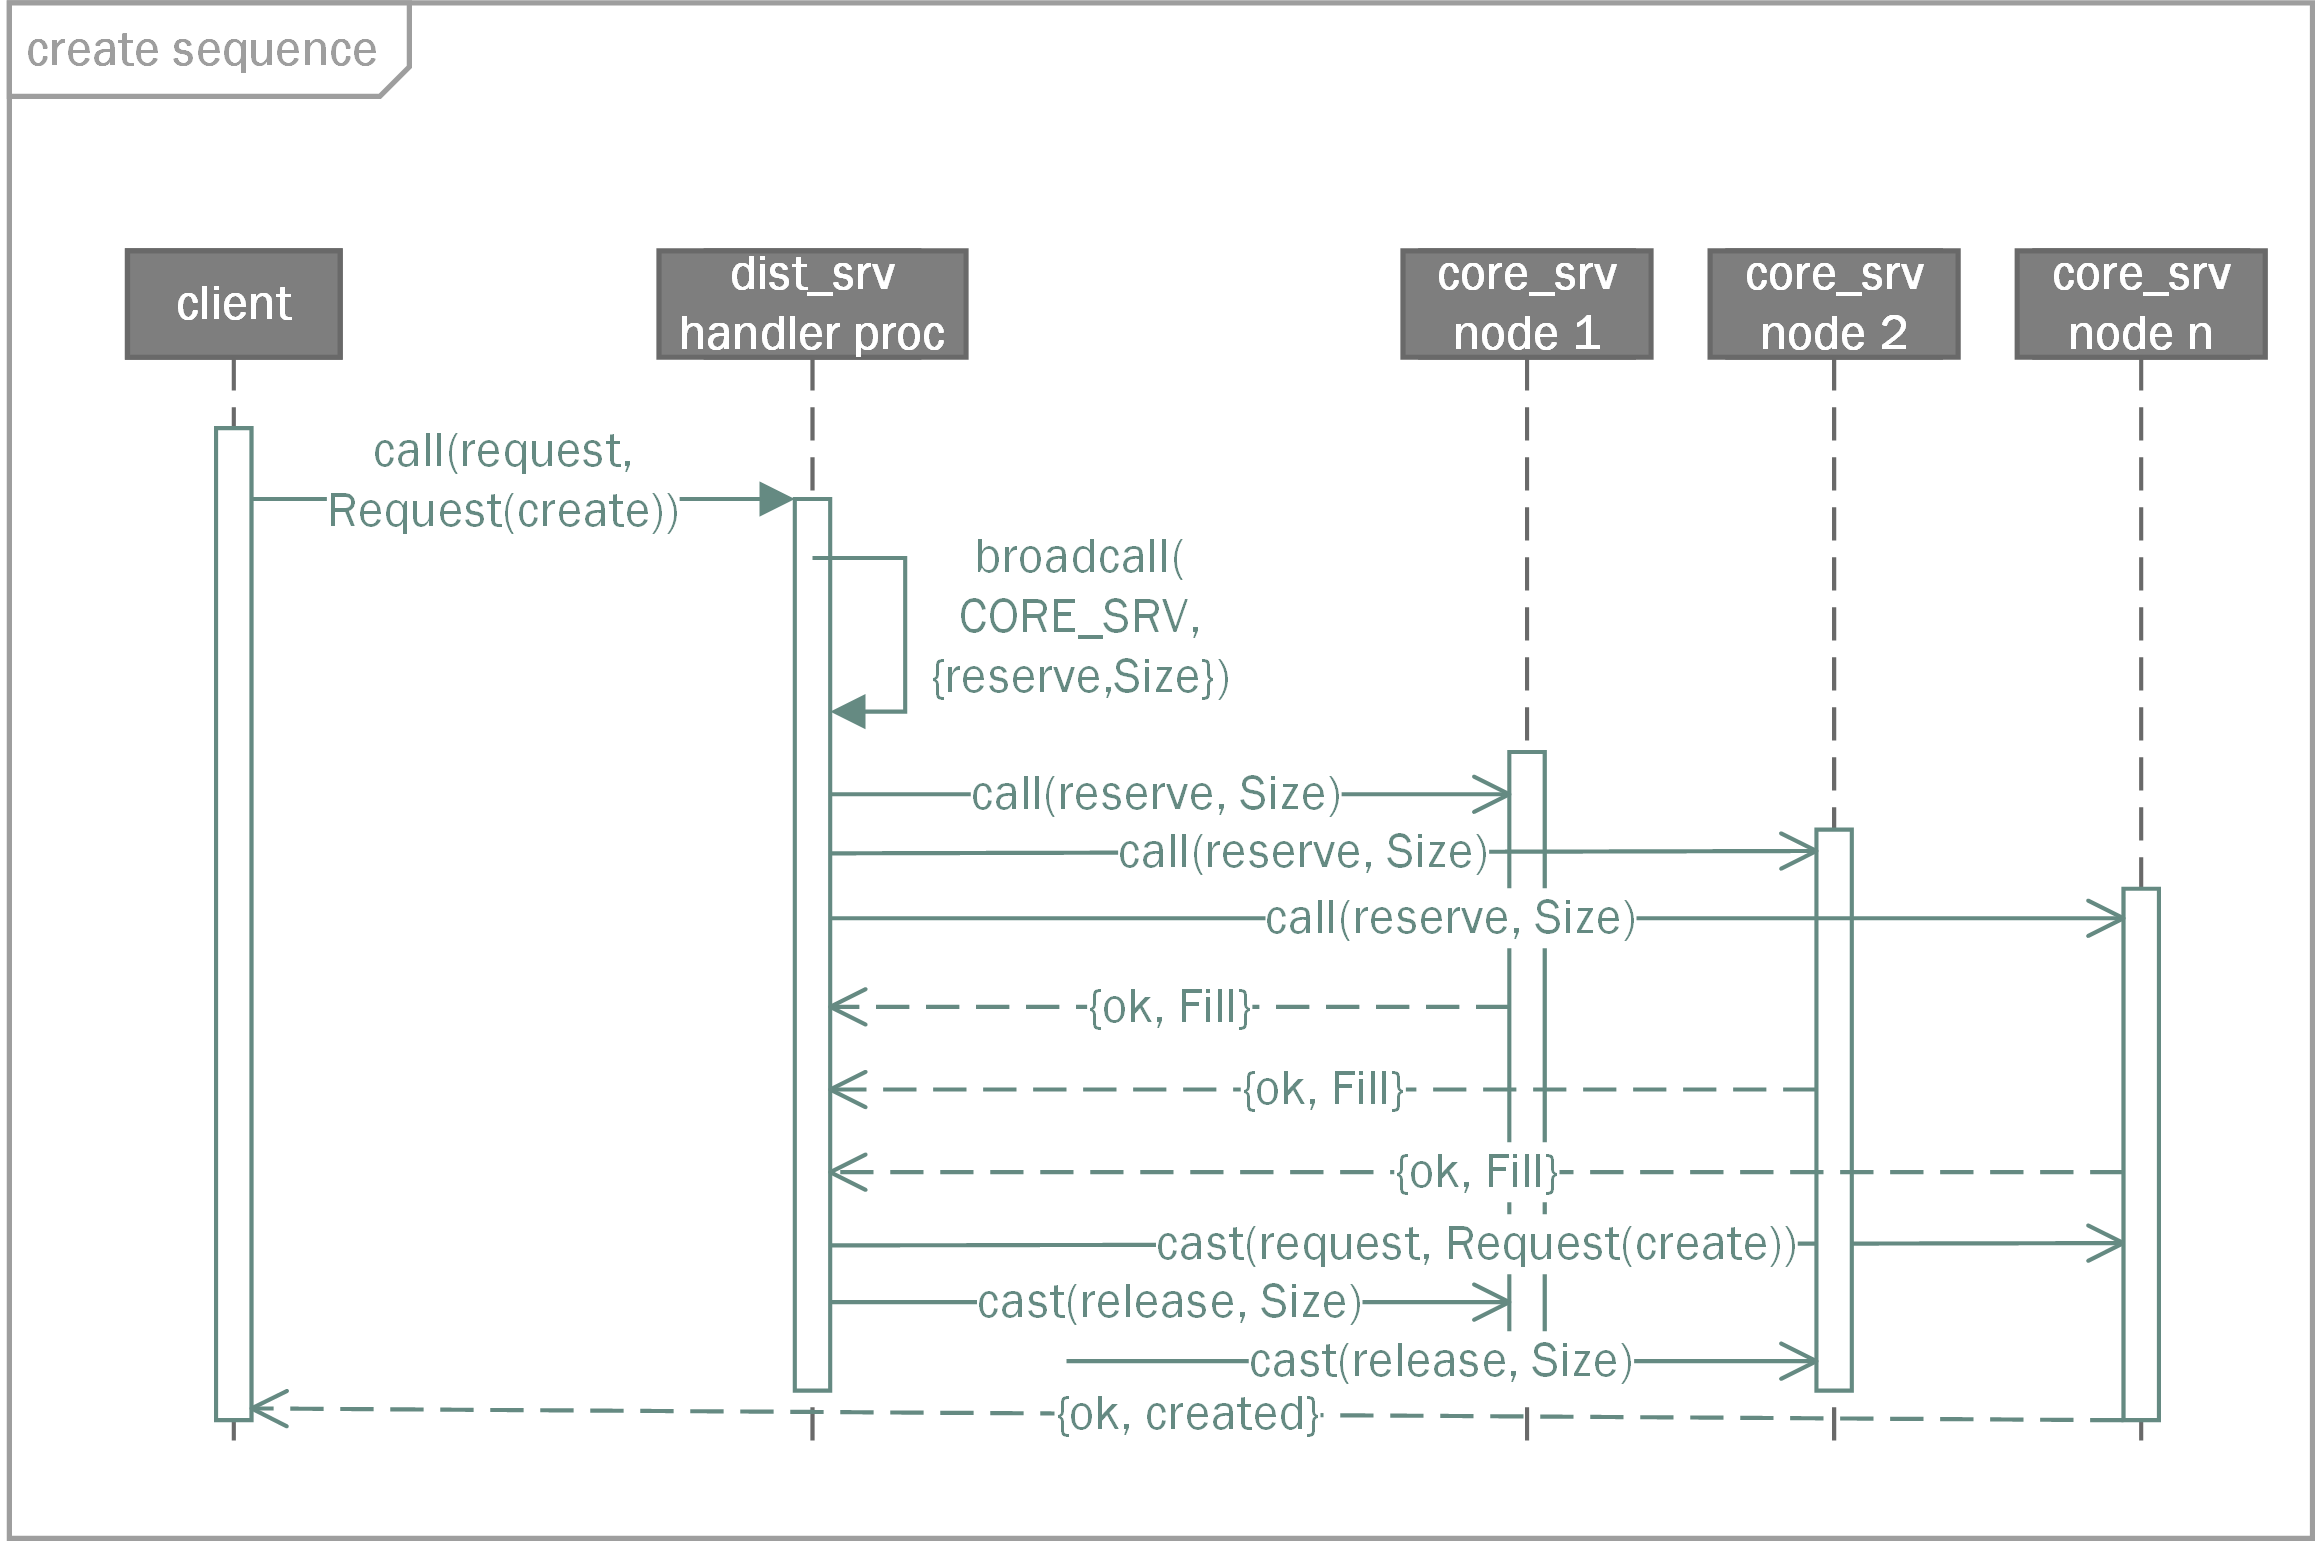
\includegraphics[width=0.9\textwidth]{dist-create-seq}
	\caption[Zapytanie \textit{create} w module komunikacyjnym.]{Obsługa zapytania create. Następuje rezerwacja miejsca na wszystkich węzłach, wybierany jest najbardziej odpowiedni do przechowania pliku, a zarezerwowane miejsce jest zwalniane.}
	\label{fig:dist-create-seq}
\end{figure}


\paragraph{Obsługa zapytań update}
Zapytanie update przekazywane jest bezpośrednio do węzła który przechowuje aktualizowany plik. Implementacja wykorzystuje dodatkowe zapytanie find, w celu zlokalizowania tego węzła. Sekwencja jest więc bardzo podobna do tej przedstawionej na \autoref{fig:dist-seq}.
